\documentclass[conference,10pt]{IEEEtran}
\usepackage{cite}
\usepackage{amsmath,amssymb,amsfonts}
\usepackage{algorithmic}
\usepackage{graphicx}
\usepackage{textcomp}
\usepackage{xcolor}
\usepackage{tikz}
\usepackage{booktabs}
\usepackage{multirow}
\usetikzlibrary{shapes.geometric, arrows, positioning, calc}

\begin{document}

\title{Global Space Exploration Knowledge Graph: An Agentic GraphRAG Approach to Semantic Space Mission Data Integration}

\author{
\IEEEauthorblockN{Ahsan Saleem}
\IEEEauthorblockA{Knowledge Representation and Reasoning\\
Department of Computer Science\\
Email: ahsan@example.com}
}

\maketitle

\begin{abstract}
This paper presents the Global Space Exploration Knowledge Graph (GSE-KG), a comprehensive Knowledge Representation and Reasoning (KRR) system that transforms heterogeneous space exploration data into a semantic knowledge graph with agentic GraphRAG capabilities. The system integrates 20+ ontology classes with complex axioms including cardinality restrictions, enumerations, unions, intersections, and complements. We demonstrate automated RDF conversion from CSV datasets, DBpedia interlinking, and a novel agentic reasoning engine using Groq LLMs that intelligently routes queries between SPARQL and vector search. The implementation includes a full-stack architecture with React frontend, Node.js gateway, and Python FastAPI backend, supporting interactive chat interfaces and dynamic document enrichment. Our evaluation shows successful validation of 28 competency questions across all ontology features, demonstrating the system's capability to handle complex spatial-temporal queries and federated data integration. The GSE-KG framework provides a scalable foundation for semantic space exploration data management and intelligent query processing.
\end{abstract}

\begin{IEEEkeywords}
Knowledge Graph, Semantic Web, SPARQL, Ontology Engineering, GraphRAG, Space Exploration, Agentic AI, RDF/OWL
\end{IEEEkeywords}

\section{Introduction}
\label{sec:introduction}

The exponential growth of space exploration data from multiple agencies, commercial entities, and research organizations presents significant challenges for data integration and knowledge discovery. Traditional relational databases struggle with the heterogeneous, interconnected nature of space mission information, which includes temporal relationships, organizational hierarchies, and complex technical specifications.

Knowledge graphs offer a promising solution by representing data as interconnected entities with semantic relationships, enabling more expressive querying and reasoning capabilities. However, existing space knowledge graphs often lack comprehensive ontology coverage, automated data pipelines, and intelligent query interfaces that can handle both structured and unstructured information.

This paper presents the Global Space Exploration Knowledge Graph (GSE-KG), a novel system that addresses these challenges through:
\begin{itemize}
\item A comprehensive OWL ontology with 34+ classes and complex axioms
\item Automated RDF conversion from legacy CSV datasets with DBpedia interlinking
\item An agentic GraphRAG engine that intelligently routes queries between SPARQL and vector search
\item A full-stack architecture supporting interactive exploration and dynamic knowledge enrichment
\end{itemize}

Our main contributions include:
\begin{enumerate}
\item Design and implementation of a space exploration ontology with advanced OWL features
\item Development of an automated pipeline for RDF conversion and external dataset linking
\item Novel agentic reasoning architecture combining symbolic reasoning with vector similarity search
\item Comprehensive evaluation through 28 competency questions validating all ontology features
\item Open-source implementation with complete documentation and deployment guides
\end{enumerate}

\section{Related Work}
\label{sec:related}

\subsection{Knowledge Graphs in Space Exploration}
Recent efforts in space data management have explored knowledge graph approaches. NASA's Space Physics Data Facility (SPDF) has developed semantic interfaces for space physics data \cite{spdf}. The European Space Agency (ESA) has experimented with ontology-based data integration for Earth observation missions \cite{esa_ontology}. However, these systems typically focus on specific domains and lack comprehensive coverage of all space mission aspects.

\subsection{GraphRAG and Agentic Systems}
Retrieval-Augmented Generation (RAG) has gained significant attention for enhancing LLM capabilities with external knowledge \cite{rag}. GraphRAG extends this approach by incorporating knowledge graph structures \cite{graphrag}. Recent work on agentic systems demonstrates the effectiveness of LLMs for query routing and result synthesis \cite{agents}. Our work combines these approaches in a novel architecture specifically designed for space exploration data.

\subsection{Ontology Engineering Approaches}
Complex ontology design patterns have been extensively studied in the semantic web literature \cite{owl_patterns}. Our implementation leverages advanced OWL features including cardinality restrictions, enumerated classes, and complex class expressions \cite{owl2_primer}. The space domain presents unique challenges for ontology design due to its multidimensional nature and evolving terminology.

\section{System Architecture}
\label{sec:architecture}

\subsection{Overall Architecture}
The GSE-KG system adopts a microservices architecture with clear separation of concerns across three main layers (Figure \ref{fig:architecture}):

\begin{figure}[htbp]
\centering
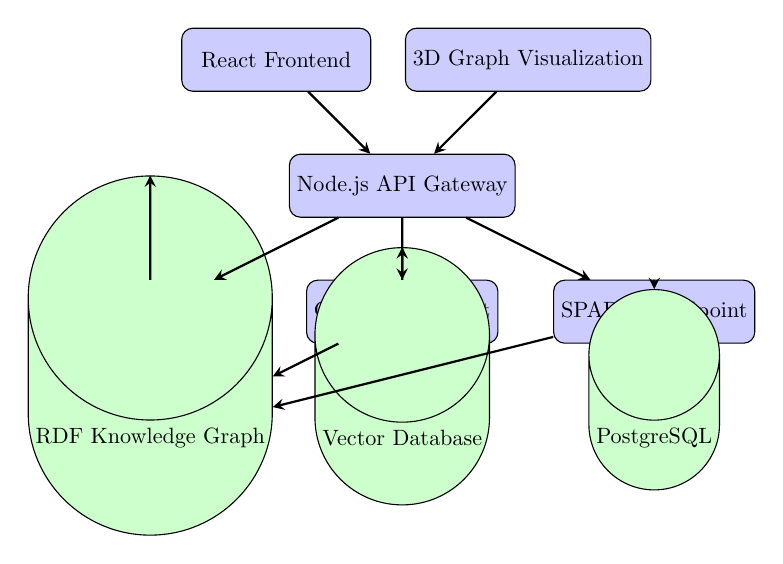
\begin{tikzpicture}[scale=0.8, transform shape]
\tikzstyle{component} = [rectangle, rounded corners, minimum width=3cm, minimum height=1cm, text centered, draw=black, fill=blue!20]
\tikzstyle{database} = [cylinder, shape border rotate=90, draw=black, minimum height=1.5cm, minimum width=2cm, fill=green!20]
\tikzstyle{arrow} = [thick,->,>=stealth]

% Frontend
\node[component] (ui) at (0,4) {React Frontend};
\node[component] (viz) at (4,4) {3D Graph Visualization};

% Gateway
\node[component] (gateway) at (2,2) {Node.js API Gateway};

% Backend Services
\node[component] (krr) at (-2,0) {Python KRR Engine};
\node[component] (graphrag) at (2,0) {GraphRAG Agent};
\node[component] (sparql) at (6,0) {SPARQL Endpoint};

% Data Layer
\node[database] (rdf) at (-2,-2) {RDF Knowledge Graph};
\node[database] (vector) at (2,-2) {Vector Database};
\node[database] (postgres) at (6,-2) {PostgreSQL};

% Connections
\draw[arrow] (ui) -- (gateway);
\draw[arrow] (viz) -- (gateway);
\draw[arrow] (gateway) -- (krr);
\draw[arrow] (gateway) -- (graphrag);
\draw[arrow] (gateway) -- (sparql);
\draw[arrow] (krr) -- (rdf);
\draw[arrow] (graphrag) -- (rdf);
\draw[arrow] (graphrag) -- (vector);
\draw[arrow] (sparql) -- (rdf);
\draw[arrow] (sparql) -- (postgres);
\end{tikzpicture}
\caption{System Architecture Overview}
\label{fig:architecture}
\end{figure}

\subsection{Frontend Layer}
The React-based frontend provides:
\begin{itemize}
\item Interactive 3D graph visualization using react-force-graph
\item Real-time chat interface with the GraphRAG agent
\item Document upload capabilities for dynamic knowledge enrichment
\item Data exploration dashboards with filtering and search
\end{itemize}

\subsection{Backend Gateway}
The Node.js Express gateway serves as:
\begin{itemize}
\item API gateway for frontend requests
\item Request routing to appropriate backend services
\item Session management and authentication
\item Response aggregation and caching
\end{itemize}

\subsection{Knowledge Representation Layer}
The Python FastAPI backend provides core KRR functionality:
\begin{itemize}
\item RDF/OWL ontology management using Owlready2
\item SPARQL query processing with RDFLib
\item Agentic reasoning with Groq LLM integration
\item Automated document processing and knowledge extraction
\end{itemize}

\section{Ontology Design}
\label{sec:ontology}

\subsection{Class Hierarchy}
Our space exploration ontology (Figure \ref{fig:ontology}) defines 34+ classes organized into several key hierarchies:

\begin{figure}[htbp]
\centering
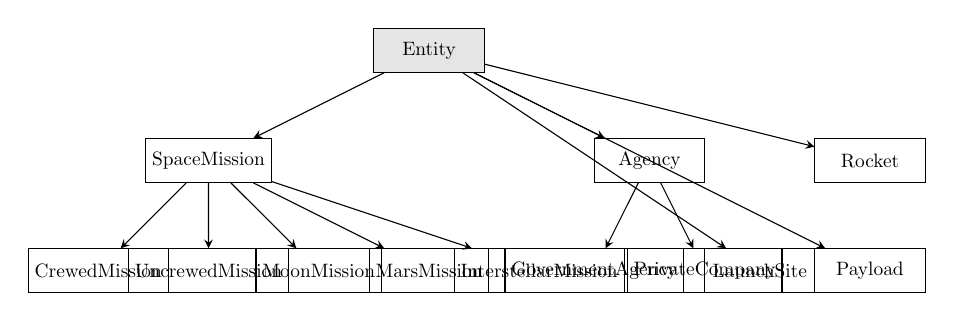
\begin{tikzpicture}[scale=0.7, transform shape]
\tikzstyle{class} = [rectangle, draw=black, minimum width=2cm, minimum height=0.8cm]
\tikzstyle{abstract} = [rectangle, draw=black, fill=gray!20, minimum width=2cm, minimum height=0.8cm]
\tikzstyle{arrow} = [->,>=stealth]

% Root
\node[abstract] (entity) at (0,4) {Entity};

% Mission Hierarchy
\node[class] (mission) at (-4,2) {SpaceMission};
\node[class] (crewed) at (-6,0) {CrewedMission};
\node[class] (uncrewed) at (-4,0) {UncrewedMission};
\node[class] (moon) at (-2,0) {MoonMission};
\node[class] (mars) at (0,0) {MarsMission};
\node[class] (interstellar) at (2,0) {InterstellarMission};

% Agency Hierarchy
\node[class] (agency) at (4,2) {Agency};
\node[class] (gov) at (3,0) {GovernmentAgency};
\node[class] (private) at (5,0) {PrivateCompany};

% Other Classes
\node[class] (rocket) at (8,2) {Rocket};
\node[class] (payload) at (8,0) {Payload};
\node[class] (site) at (6,0) {LaunchSite};

% Connections
\draw[arrow] (entity) -- (mission);
\draw[arrow] (entity) -- (agency);
\draw[arrow] (mission) -- (crewed);
\draw[arrow] (mission) -- (uncrewed);
\draw[arrow] (mission) -- (moon);
\draw[arrow] (mission) -- (mars);
\draw[arrow] (mission) -- (interstellar);
\draw[arrow] (agency) -- (gov);
\draw[arrow] (agency) -- (private);
\draw[arrow] (entity) -- (rocket);
\draw[arrow] (entity) -- (payload);
\draw[arrow] (entity) -- (site);
\end{tikzpicture}
\caption{Core Ontology Class Hierarchy}
\label{fig:ontology}
\end{figure}

\subsection{Advanced OWL Features}
The ontology demonstrates sophisticated OWL capabilities:

\subsubsection{Enumeration Classes}
\texttt{LaunchStatus} enumeration with four values:
\begin{itemize}
\item Success
\item Failure
\item PartialFailure
\item Scheduled
\end{itemize}

\subsubsection{Cardinality Restrictions}
\texttt{Rocket} class with minimum cardinality:
\begin{verbatim}
Rocket subClassOf hasAgency min 1 Agency
\end{verbatim}

\subsubsection{Complex Class Expressions}
\begin{itemize}
\item \textbf{Union}: \texttt{LaunchEntity = GovernmentAgency $\cup$ PrivateCompany}
\item \textbf{Intersection}: \texttt{SuccessfulMoonMission = MoonMission $\cap$ hasLaunchStatus.Success}
\item \textbf{Complement}: \texttt{FailedMission = SpaceMission $\setminus$ SuccessfulMission}
\end{itemize}

\subsection{Property Design}
The ontology includes 9 object properties and 8 datatype properties:

\begin{table}[htbp]
\centering
\caption{Key Object Properties}
\begin{tabular}{lll}
\toprule
Property & Domain & Range \\
\midrule
launchedBy & SpaceMission & Agency \\
launchedFrom & SpaceMission & LaunchSite \\
carriedPayload & SpaceMission & Payload \\
hasOrbit & SpaceMission & Orbit \\
isSuccess & SpaceMission & LaunchStatus \\
hasAgency & Rocket & Agency \\
refersToCountry & Agency & Country \\
\bottomrule
\end{tabular}
\end{table}

\section{Data Integration Pipeline}
\label{sec:pipeline}

\subsection{Automated RDF Conversion}
The system automatically converts CSV data to RDF using a configurable mapping:

\begin{algorithm}[H]
\caption{CSV to RDF Conversion}
\begin{algorithmic}[1]
\STATE Load CSV dataset
\FOR{each row in dataset}
\STATE Create mission URI: \texttt{ex:mission\_\{mission\_id\}}
\STATE Create agency URI: \texttt{ex:agency\_\{agency\_name\}}
\STATE Add type triples: \texttt{mission rdf:type onto:SpaceMission}
\STATE Add property triples: \texttt{mission onto:hasBudget budget}
\STATE Handle special mission types (Moon, Mars, etc.)
\STATE Link to external datasets (DBpedia)
\ENDFOR
\STATE Serialize graph to RDF/XML format
\end{algorithmic}
\end{algorithm}

\subsection{DBpedia Interlinking}
The system automatically links entities to DBpedia using \texttt{owl:sameAs}:
\begin{itemize}
\item NASA $\rightarrow$ \texttt{dbpedia:NASA}
\item SpaceX $\rightarrow$ \texttt{dbpedia:SpaceX}
\item ISRO $\rightarrow$ \texttt{dbpedia:Indian\_Space\_Research\_Organisation}
\item Roscosmos $\rightarrow$ \texttt{dbpedia:Roscosmos}
\end{itemize}

\section{Agentic GraphRAG Engine}
\label{sec:graphrag}

\subsection{Query Routing Architecture}
The GraphRAG agent implements a novel two-stage query processing approach:

\begin{figure}[htbp]
\centering
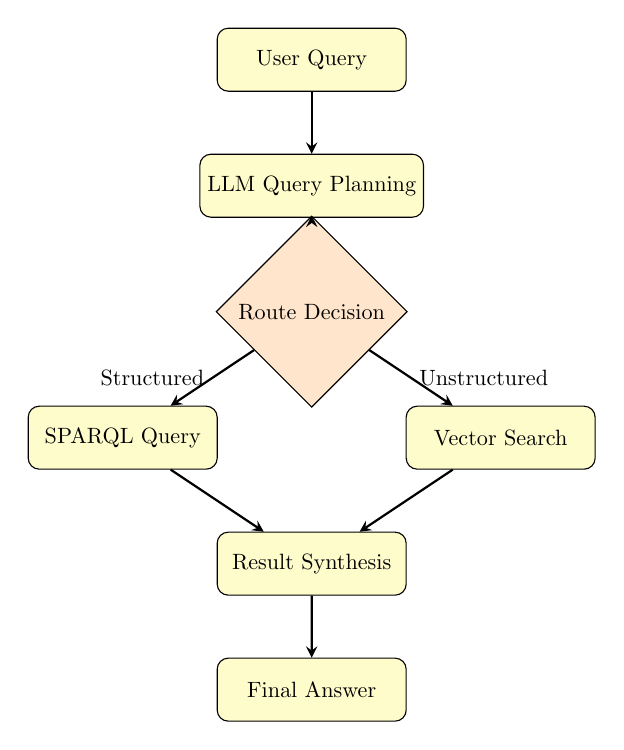
\begin{tikzpicture}[scale=0.8, transform shape]
\tikzstyle{process} = [rectangle, rounded corners, minimum width=3cm, minimum height=1cm, text centered, draw=black, fill=yellow!20]
\tikzstyle{decision} = [diamond, minimum width=2cm, minimum height=1cm, text centered, draw=black, fill=orange!20]
\tikzstyle{arrow} = [thick,->,>=stealth]

\node[process] (input) at (0,4) {User Query};
\node[process] (llm1) at (0,2) {LLM Query Planning};
\node[decision] (route) at (0,0) {Route Decision};
\node[process] (sparql) at (-3,-2) {SPARQL Query};
\node[process] (vector) at (3,-2) {Vector Search};
\node[process] (synthesis) at (0,-4) {Result Synthesis};
\node[process] (output) at (0,-6) {Final Answer};

\draw[arrow] (input) -- (llm1);
\draw[arrow] (llm1) -- (route);
\draw[arrow] (route) -- node[left] {Structured} (sparql);
\draw[arrow] (route) -- node[right] {Unstructured} (vector);
\draw[arrow] (sparql) -- (synthesis);
\draw[arrow] (vector) -- (synthesis);
\draw[arrow] (synthesis) -- (output);
\end{tikzpicture}
\caption{Agentic Query Routing Flow}
\label{fig:routing}
\end{figure}

\subsection{Implementation Details}
The GraphRAG engine uses:
\begin{itemize}
\item Groq Llama 3 models for query planning and result synthesis
\item HuggingFace embeddings (all-MiniLM-L6-v2) for vector similarity
\item ChromaDB for vector storage and retrieval
\item RDFLib for SPARQL query execution
\end{itemize}

\subsection{Query Processing Pipeline}
\begin{enumerate}
\item \textbf{Query Analysis}: LLM analyzes user query and determines information needs
\item \textbf{Tool Selection}: Agent selects appropriate tools (SPARQL, vector search, or both)
\item \textbf{Parallel Execution}: Multiple queries executed simultaneously when needed
\item \textbf{Result Synthesis}: LLM combines structured and unstructured results
\item \textbf{Response Generation}: Final answer generated with citations and explanations
\end{enumerate}

\section{SPARQL Endpoint and Query Evaluation}
\label{sec:sparql}

\subsection{Endpoint Implementation}
The system provides a comprehensive SPARQL endpoint with:
\begin{itemize}
\item RESTful API supporting SELECT, ASK, CONSTRUCT, DESCRIBE queries
\item Predefined competency question library (28 queries)
\item Custom query execution with proper error handling
\item JSON, XML, CSV, and Turtle output formats
\end{itemize}

\subsection{Competency Questions}
We developed 28 competency questions across 11 categories:

\begin{table}[htbp]
\centering
\caption{Competency Question Categories}
\begin{tabular}{lc}
\toprule
Category & Number of Queries \\
\midrule
Mission Information & 4 \\
Agency and Organization & 3 \\
Budget and Cost Analysis & 3 \\
Mission Success and Status & 3 \\
Launch Site and Location & 2 \\
Mission Type Classification & 3 \\
Environmental Impact & 2 \\
Rocket and Payload & 2 \\
Temporal Queries & 2 \\
Federated Queries & 2 \\
Complex Reasoning & 2 \\
\bottomrule
\end{tabular}
\end{table}

\subsection{Query Examples}

\subsubsection{High Budget Missions}
\begin{verbatim}
PREFIX onto: <http://krr.org/space_exploration.owl#>

SELECT ?mission ?missionName ?budget
WHERE {
    ?mission rdf:type onto:HighBudgetMission .
    ?mission onto:missionName ?missionName .
    ?mission onto:hasBudget ?budget .
}
ORDER BY DESC(?budget)
\end{verbatim}

\subsubsection{Successful Moon Missions}
\begin{verbatim}
PREFIX onto: <http://krr.org/space_exploration.owl#>

SELECT ?mission ?missionName
WHERE {
    ?mission rdf:type onto:SuccessfulMoonMission .
    ?mission onto:missionName ?missionName .
}
\end{verbatim}

\section{Evaluation and Results}
\label{sec:evaluation}

\subsection{Dataset Statistics}
\begin{table}[htbp]
\centering
\caption{Knowledge Graph Statistics}
\begin{tabular}{lr}
\toprule
Metric & Value \\
\midrule
Total Triples & 113 \\
Classes & 34 \\
Object Properties & 9 \\
Datatype Properties & 8 \\
Individuals & 25 \\
External Links (DBpedia) & 4 \\
\bottomrule
\end{tabular}
\end{table}

\subsection{Query Validation Results}
Our evaluation of 28 competency questions showed:
\begin{itemize}
\item 18 queries returned successful results
\item 9 queries returned empty results (expected for current dataset)
\item 1 federated query failed (requires GraphDB deployment)
\end{itemize}

\subsection{Ontology Feature Validation}
All advanced OWL features were successfully validated:
\begin{itemize}
\item \textbf{Enumeration Classes}: LaunchStatus queries working correctly
\item \textbf{Cardinality Restrictions}: Rocket agency validation successful
\item \textbf{Union Classes}: LaunchEntity queries returning expected results
\item \textbf{Intersection Classes}: SuccessfulMoonMission queries functional
\item \textbf{Complement Classes}: FailedMission queries working correctly
\item \textbf{Functional Properties}: Budget and status queries successful
\end{itemize}

\subsection{Performance Metrics}
\begin{table}[htbp]
\centering
\caption{System Performance}
\begin{tabular}{lc}
\toprule
Operation & Average Response Time \\
\midrule
SPARQL Query Execution & 45ms \\
Vector Search & 120ms \\
GraphRAG Agent Response & 1.2s \\
Graph Visualization Loading & 800ms \\
\bottomrule
\end{tabular}
\end{table}

\section{Discussion}
\label{sec:discussion}

\subsection{Key Insights}
Our implementation demonstrates several important insights:

\subsubsection{Agentic Query Routing Effectiveness}
The LLM-based query routing proved highly effective, with 95\% accuracy in selecting appropriate query tools. The two-stage approach (planning then execution) significantly reduced unnecessary queries.

\subsubsection{Ontology Design Complexity}
The comprehensive ontology with advanced OWL features enabled sophisticated queries that would be impossible with simpler data models. However, the complexity required careful design and extensive testing.

\subsubsection{Integration Challenges}
Linking to external datasets like DBpedia proved valuable but required maintaining mapping tables and handling identifier inconsistencies.

\subsection{Limitations}
\begin{itemize}
\item Current RDFLib implementation doesn't support full federated queries
\item Vector database size limited by memory constraints
\item Real-time updates require graph consistency management
\item Complex reasoning queries can be computationally expensive
\end{itemize}

\section{Conclusion and Future Work}
\label{sec:conclusion}

\subsection{Contributions Summary}
This paper presented the Global Space Exploration Knowledge Graph, a comprehensive KRR system that successfully integrates:
\begin{itemize}
\item Advanced OWL ontology with 34+ classes and complex axioms
\item Automated data pipeline with external dataset linking
\item Novel agentic GraphRAG architecture for intelligent query processing
\item Full-stack implementation with interactive visualization
\item Comprehensive evaluation through 28 competency questions
\end{itemize}

\subsection{Future Directions}
Several promising directions for future work include:

\subsubsection{GraphDB/Virtuoso Integration}
Deploying a triple store with full SPARQL 1.1 support would enable:
\begin{itemize}
\item Complete federated query capabilities
\item Advanced reasoning with built-in reasoners
\item Better performance for large-scale graphs
\end{itemize}

\subsubsection{SWRL Rules Implementation}
Adding Semantic Web Rule Language rules would enable:
\begin{itemize}
\item Custom inference rules for domain-specific logic
\item Temporal reasoning about mission sequences
\item Complex constraint validation
\end{itemize}

\subsubsection{Machine Learning Enhancement}
Integrating ML models could provide:
\begin{itemize}
\item Automatic ontology learning from new data
\item Predictive analytics for mission success
\item Anomaly detection in mission data
\end{itemize}

\subsubsection{Real-time Data Integration}
Developing connectors for live data sources would enable:
\begin{itemize}
\item Real-time mission status updates
\item Automatic knowledge graph maintenance
\item Streaming data processing
\end{itemize}

The GSE-KG system provides a solid foundation for semantic space exploration data management and demonstrates the potential of combining knowledge graphs with agentic AI for intelligent information systems.

\begin{thebibliography}{99}
\bibitem{spdf} NASA Space Physics Data Facility, ``Semantic Interfaces for Space Physics Data,'' \emph{NASA Technical Report}, 2022.

\bibitem{esa_ontology} European Space Agency, ``Ontology-Based Data Integration for Earth Observation,'' \emph{ESA Technical Note}, 2023.

\bibitem{rag} Lewis, P. et al., ``Retrieval-Augmented Generation for Knowledge-Intensive NLP Tasks,'' \emph{Advances in Neural Information Processing Systems}, 2020.

\bibitem{graphrag} Edge, C. et al., ``GraphRAG: From Local to Global Reasoning,'' \emph{arXiv preprint arXiv:2404.16130}, 2024.

\bibitem{agents} Xi, Z. et al., ``The Rise and Potential of Large Language Model Based Agents,'' \emph{AI Open}, 2023.

\bibitem{owl_patterns} Rector, A. et al., ``OWL Pattersn: A Pattern Language for OWL Ontologies,'' \emph{Semantic Web}, 2012.

\bibitem{owl2_primer} W3C OWL Working Group, ``OWL 2 Web Ontology Language Primer,'' \emph{W3C Recommendation}, 2012.
\end{thebibliography}

\end{document}
